\section{本章の概要}
本章では,学習者理解度可視化システムとしてのシステムにおける具体的な実行手順と,実行手順の中で使用される機能についての詳細を述べる.

\section{システム実行の流れ}
\subsection{前提条件}
本システムを実行する前に満たすべき前提条件を示す.
まず,本システムは全てDocker上で動作するため,Dockerを使用できるPC上でのみ動作する.
そのPCの必要最低動作環境を表\ref{tab:docker_env}に示す.
\newpage
\begin{table}[htb]
    \centering
    \caption{Dockerのシステム要件}
    \label{tab:docker_env}
    \begin{tabular}{|c|c|}  \hline
        \multirow{5}{*}{Windows} & Windows 10 64 ビット:Pro、Enterprise、Education(ビルド 15063 以上) \\
		              & Hyper-V と Windows コンテナ機能の有効化 \\ 
                      & 64 ビット SLAT (Second Level Address Translation) 対応プロセッサ \\ 
                      & 4GB システムメモリ \\ 
                      & BIOS レベルでのハードウェア仮想化の有効化 \\ \hline
        \multirow{2}{*}{Intel チップの Mac} & macOS はバージョン 10.15 またはそれ以降 \\
        & 最小 4GB の メモリ RAM \\ \hline
        Apple silicon の Mac & Rosetta 2 のインストール \\ \hline
        \multirow{7}{*}{Linux系} & 仮想化のために、 64-bit カーネルと CPU のサポート \\
        & KVM 仮想化のサポート \\ 
        & QEMUバージョン5.2以上 \\
        & systemd init システム \\ 
        & Gnome または KDE デスクトップ環境 \\ 
        & 最小 4GB の メモリ RAM \\
        & ユーザ名前空間で ID マッピングの設定を有効化 \\ \hline
    \end{tabular}
\end{table}

以上の条件を満たすPC上でDockerをインストールすることにより,本システムは使用できる.
\newpage

\subsection{システム実行の流れ}
本節では,システム実行の流れについて説明する.
本システムの利用者は学習者とそれを指導する指導者となるため,両者それぞれのシステム実行の流れを説明する.
\subsubsection{指導者}
指導者は本システムを立ち上げて学習者が本システムを利用できるようにしなければならない.
まず,指導者は本システムをWebサーバーにインストールし,dockerコマンドを用いて本システムサーバを立ち上げる.
その後\url{http://127.0.0.1:7878/}にアクセスすることにより本システムにアクセスすることができる.
アクセスした直後のGUI(以下,ホーム画面)を図\ref{fig:home}に示す.

\begin{figure}[htbp]
\begin{center}
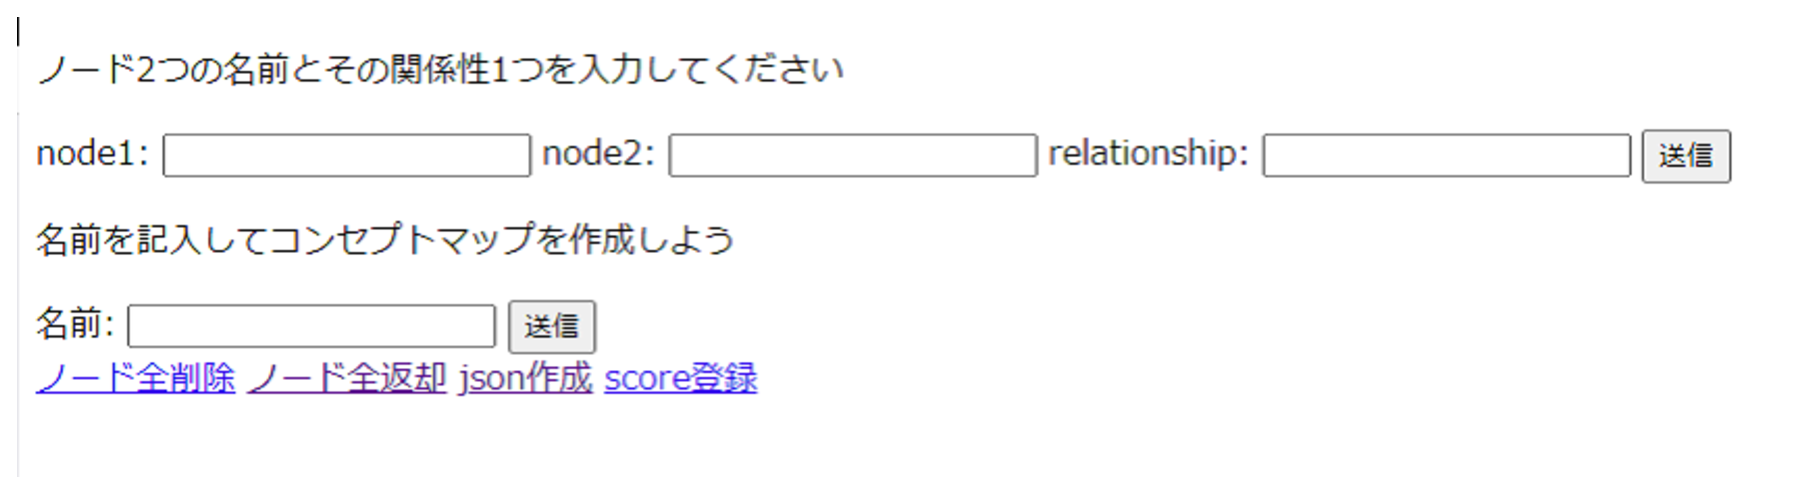
\includegraphics[width=18cm]{img/home.eps}
\end{center}
\caption{ホーム画面}
\label{fig:home}
\end{figure}

指導者はホーム画面のjson作成ボタンからグラフデータの入力を開始できる.
その後,第\ref{chap:content}章の\ref{subsec:hojo}節で示した図\ref{fig:hojo}のグラフデータ入力補助機能を用いてグラフデータを入力していく.
グラフデータの入力が完了した一例を図\ref{fig:ex_hojo}に示す.

\begin{figure}[htbp]
\begin{center}
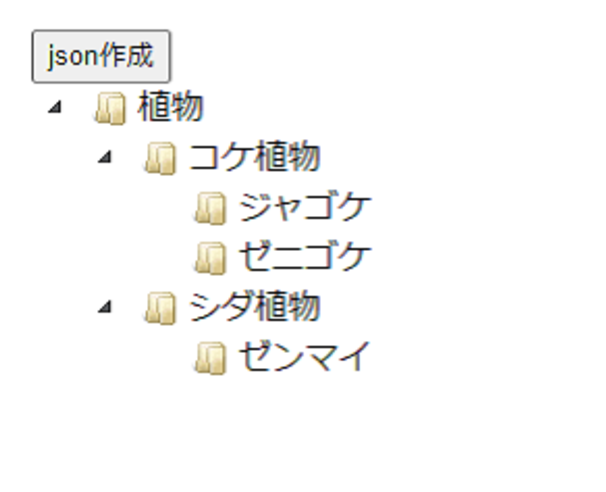
\includegraphics[width=10cm]{img/ex_hojo.eps}
\end{center}
\caption{グラフデータ入力一例}
\label{fig:ex_hojo}
\end{figure}

\newpage

グラフデータの入力が完了したらjson作成ボタンを押下する事により,グラフデータベースへデータの登録が完了する.
データが登録できたかどうかはホーム画面のノード全返却ボタンを押下して確認するか、\url{http://127.0.0.1:7474/}にアクセスすれば確認できる.
\url{http://127.0.0.1:7474/}にアクセスした際のGUIを図\ref{fig:neo4j_check}に示す.

\begin{figure}[htbp]
\begin{center}
\includegraphics[width=18cm]{img/neo4j_check.eps}
\end{center}
\caption{グラフデータ確認画面}
\label{fig:neo4j_check}
\end{figure}
\newpage

図\ref{fig:neo4j_check}のページはNeo4jが提供するページで様々なクエリを発行することによってデータを閲覧できる.
今回はMATCH文を用いて先ほど入力したグラフデータを表示した.

続いて,グラフデータの入力が完了したら指導者は学習者に対して試験を実施する.
実施後の試験の結果を本システムに登録する必要がある.
登録するにはホーム画面のscore登録ボタンから学生の成績を登録できる.
score登録のGUIを図\ref{fig:score}に示す.

\begin{figure}[htbp]
\begin{center}
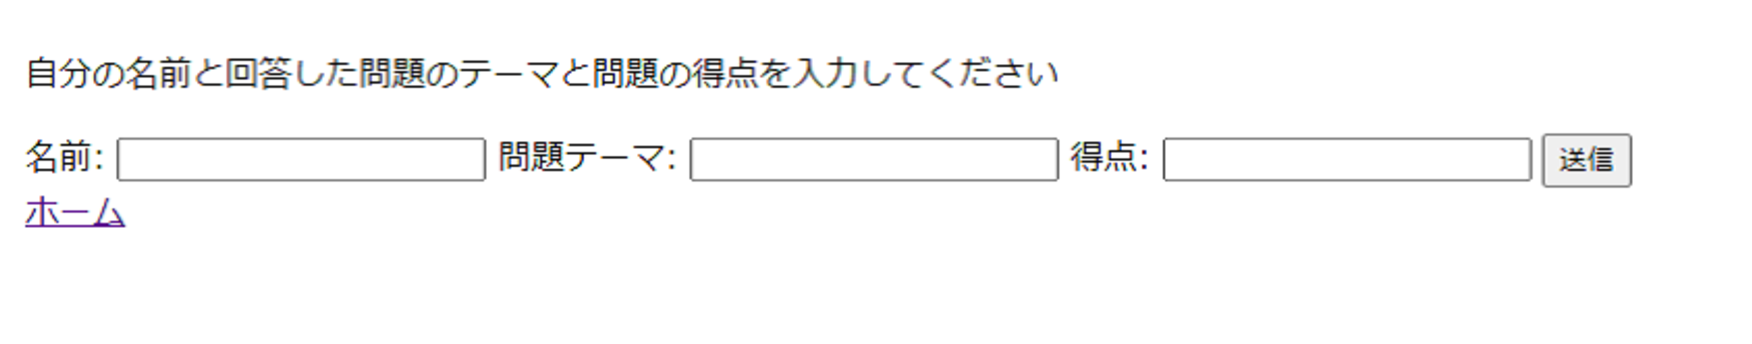
\includegraphics[width=18cm]{img/score.eps}
\end{center}
\caption{score登録画面}
\label{fig:score}
\end{figure}

このフォームでは名前の部分に学習者の名前を入力し,問題テーマに先ほど入力したグラフデータの子ノードに当たるものを入力し,得点を入力し,送信ボタンを押下することによって得点の登録が完了する.
例えば先ほど図\ref{fig:ex_hojo}で示したゼンマイの問題についてタケルという学習者が60点を取った場合は図\ref{fig:ex_score}のようにして入力する.

\begin{figure}[htbp]
\begin{center}
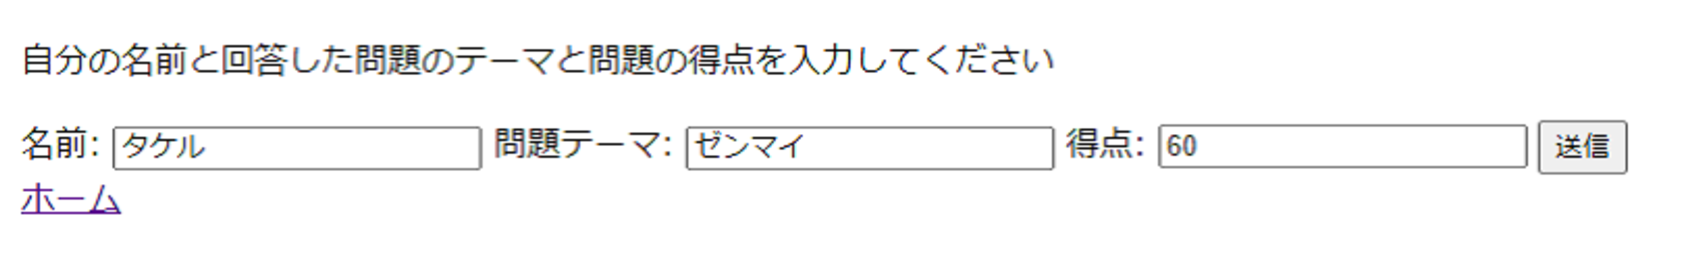
\includegraphics[width=18cm]{img/ex_score.eps}
\end{center}
\caption{score登録の一例}
\label{fig:ex_score}
\end{figure}
\newpage

\url{http://127.0.0.1:7474/}にアクセスしてデータを確認すると図\ref{fig:score_check}のようになっている.

\begin{figure}[htbp]
\begin{center}
\includegraphics[width=18cm]{img/score_check.eps}
\end{center}
\caption{score登録の確認}
\label{fig:score_check}
\end{figure}
    
図で確認できるようにタケルがゼンマイに対してscoreを持っており,そのプロパティ内のscoreが60になっていることから先ほど入力した内容が反映されていることを確認できる.

以上の手順をもって,指導者はグラフデータの入力と学習者の成績登録を本システムで実施する.
\newpage

\subsubsection{学習者}
学習者はホーム画面の名前入力フォームに自身の名前を入力すればコンセプトマップ作成画面へと移行できる.
その一例を図\ref{fig:name_enter}に示す.

\begin{figure}[htbp]
\begin{center}
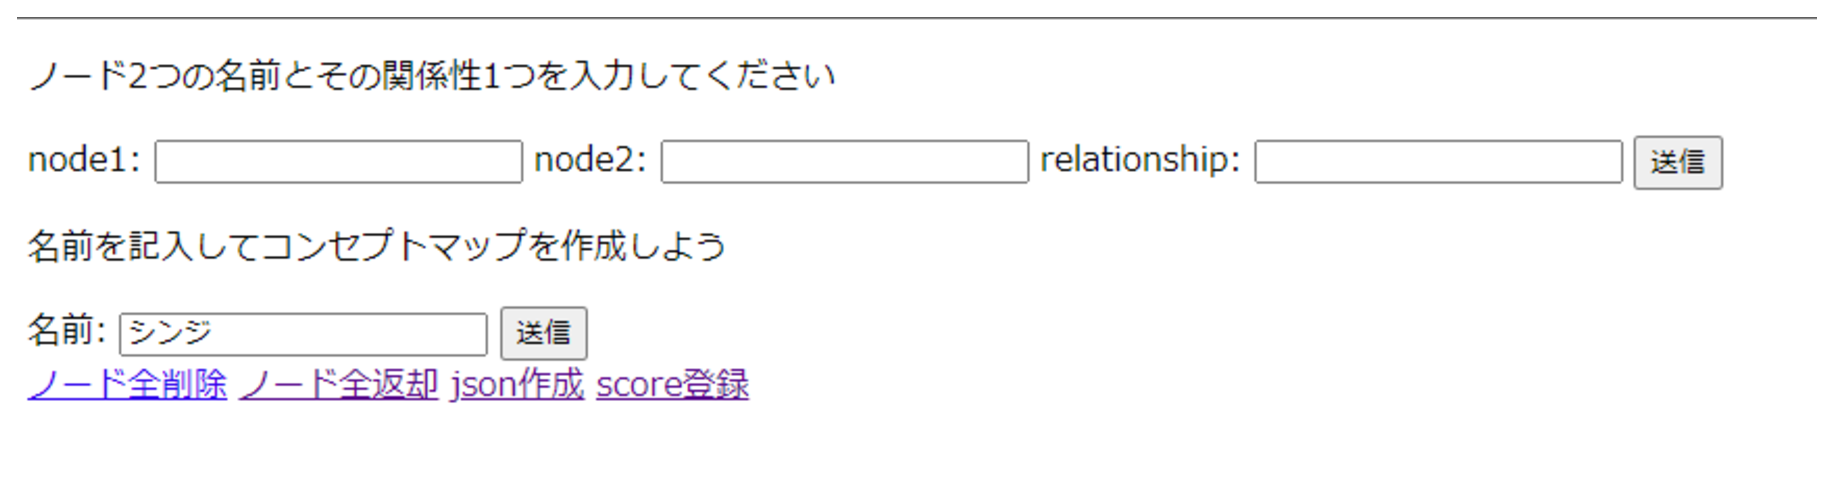
\includegraphics[width=18cm]{img/name_enter.eps}
\end{center}
\caption{名前入力画面}
\label{fig:name_enter}
\end{figure}

今回は例としてシンジという学習者が本システムを扱うこととしている.
名前入力後,シンジは図\ref{fig:sinji_concept}に示されたコンセプト作成画面へと移行できる.

\begin{figure}[htbp]
\begin{center}
\includegraphics[width=14cm]{img/sinji_concept.eps}
\end{center}
\caption{コンセプトマップ作成画面}
\label{fig:sinji_concept}
\end{figure}
\newpage

コンセプトマップ作成画面遷移後,学習者は画面に表示されているノードを表す円と円とを結線機能を用いてノード情報を確認しながら結線していく.
結線する数はedgeの数で確認し,結線する場合は画面右上の「線を引く」ボタンを押下することによって結線ができる状態に移行する.
学習者は自分が思うコンセプトマップを作成していき,最後に試験の主観的獲得点数量に基づいて,ノードをタップすることによってノードの背景色を変更できる.
背景色は獲得点数の割合が 0\%以上 25\%未満なら赤,25\%以上 50\%未満なら橙,50\%以上 75\%未満なら黄,75\%以上 100\%以下なら緑と設定できる.
背景色決定後,画面右上の「マップの答えを見る」ボタンによりコンセプトマップの答えを確認できる.
その様子を図\ref{fig:sinji_check}に示す.

\begin{figure}[htbp]
\begin{center}
\includegraphics[width=18cm]{img/kasi_system.eps}
\end{center}
\caption{コンセプトマップ確認のGUI}
\label{fig:sinji_check}
\end{figure}
\newpage

学習者はコンセプトマップ比較時に表示されているデータが邪魔であれば画面右上のすべてのデータを見るボタンを押下することによって,データの表示と非表示を選択できる.
また,ノードにマウスを重ねると一つ一つのノード情報を確認することもできる.
これらの機能を駆使して学習者は自身が作成したコンセプトマップと,システムが自動的に作成したコンセプトマップを比較することにより,
コンセプトマップの誤りがあればそれを修正し,続いてノードの背景色を比較し,自身のその分野に対する学習理解度において認識の齟齬があるかを確認し,誤りがあれば修正していく.

以上の作業で学習者は,自身が学ぶ学習分野において学習構造と学習理解度をコンセプトマップとノードの背景色をもって客観的に自身の学習理解度を認識できるため,学習目標設定の基準にできる.
